\documentclass{article}
\usepackage[
    letterpaper,
    top=0.5in,
    bottom=0.5in,
    left=1.5in,
    right=1.5in,
]{geometry}
\usepackage{amssymb,amsmath}
\usepackage{parskip}
\usepackage{fancyhdr}
\usepackage{tabularx}
\usepackage{enumerate}
\usepackage{graphicx}
\usepackage{tikz}
\usetikzlibrary{automata, positioning, arrows}
\usepackage{array}   % for \newcolumntype macro
\newcolumntype{C}{>{$}c<{$}} % math-mode version of "l" column type
% \usepackage{cmbright}
\renewcommand{\baselinestretch}{1.3}
\pagestyle{fancy}
\fancyfoot{}
\renewcommand{\headrulewidth}{0em}
\setlength{\headheight}{0.5in}
\fancypagestyle{firstpage}{
\fancyhead{}
\fancyfoot{}
}
\newcommand{\HomeworkNo}{1}
\newcommand{\MyName}{Amy M. Liu}
\newcommand{\MyPennKey}{liuamy05}
\fancyhead[L]{\MyName}
\fancyhead[R]{Homework \HomeworkNo{}}
\newcommand{\PrintFirstHeader}{
\begin{center}
CIS 2620 Summer 2025 \vspace{0.5em} \hfill {\Large{\MyName}}
\\
{\LARGE{\textbf{Homework \HomeworkNo{}}}} \vspace{0.5em} \\
PennKey: \MyPennKey \\
Collaborators:
\end{center}
}
\tikzset{
    auto,
    on grid,
    initial text=$ $,
    shorten >=1pt,
    node distance=2cm, 
    accepting/.style={fill=red!25, double},
}

\begin{document}
\thispagestyle{firstpage}
\PrintFirstHeader{}
\begin{enumerate}[\bf P1.]
\setlength\itemsep{1em}

\item
The given language is:
\[
L = \{x \in \{0,1\}^* : \text{ the number of occurences of 01 in x is same as that of 10}\} \\
\]

We will define our DFA in the following form:
\[
\mathbb{M} = \{\mathbb{Q}, \Sigma, \delta, q_0, \mathbb{F}\}
\]

The respective variables are:
\[
\begin{aligned}
\mathbb{Q} :=& \{ q_0, q_1, q_2, q_3, q_4\} \\
\Sigma :=& \{0, 1\} \\
q_0 :=& q_0 \\
\mathbb{F} :=& \{q_0\} \\
\end{aligned}
\]

The transition function is laid out below:
\begin{figure}[ht]
\centering
\begin{tabular}{ C | C C }
    \multicolumn{3}{C}{\boldsymbol{\delta := \delta(q, \sigma) : \mathbb{Q} \times \Sigma}} \\
    \hline
    \textbf{q} & \boldsymbol{\delta : \sigma = 0} & \boldsymbol{\delta : \sigma = 1} \\
    q_0 & q_1 & q_2 \\
    q_1 & q_1 & q_3 \\ 
    q_2 & q_4 & q_2 \\
    q_3 & q_1 & q_3 \\
    q_4 & q_4 & q_2 \\
\end{tabular}
\end{figure}

\textbf{Overall DFA diagram:}
\begin{figure}[ht]
    \centering
    \begin{tikzpicture}
        \node[state, accepting, initial] (q0) {q0};
        \node[state, accepting, right of=q0] (q1) {q1};
        \node[state, accepting, below of=q1] (q2) {q2};
        \node[state, right of=q1] (q3) {$q_3$};
        \node[state, below of=q3] (q4) {$q4$};

    \path[->]
        (q0) edge node[above] {0} (q1)
            edge node {1} (q2)
        (q1) edge node {1} (q3)
            edge[loop above] node {0} ()
        (q2) edge node {0} (q4)
            edge[loop below] node {1} ()
        (q3) edge[loop above] node {1} ()
            edge[bend left] node {0} (q1) 
        (q4) edge[loop below] node {0} ()
            edge[bend left] node {1} (q2);
    \end{tikzpicture}
\end{figure}

\newpage
\item
\end{enumerate}
\end{document}